% Chapter 1
\chapter{مقدمه}

در سال‌های اخیر اینترنت اشیاء\LTRfootnote { Internet Of Things } به سرعت در حال توسعه است و قابلیت‌های حساس و محاسبه فراگیر را برای اتصال طیف گسترده‌ای از وسایل به یکدیگر بر پایه اینترنت فراهم می‌کند\cite{b7}. برای رسیدن به اهداف متنوع در رابطه با داده‌های تولید شده توسط دستگاه‌های اینترنت اشیاء فراگیر، تکنیک‌های هوش مصنوعی\LTRfootnote { Artificial Intelligence } مانند یادگیری عمیق\LTRfootnote { Deep Learning } به طور گسترده‌ای برای آموزش مدل‌های داده برای فعال کردن برنامه‌های  اینترنت اشیاء  هوشمند مانند بهداشت هوشمند، حمل و نقل هوشمند و شهر هوشمند استفاده شده است\cite{b8}. به طور سنتی، عملکردهای هوش مصنوعی در یک سرور ابری یا یک مرکز داده برای یادگیری و جدا کردن داده قرار می‌گیرد که این مدل امروزه با توجه به انفجار داده  اینترنت اشیاء، محدودیت‌های بحرانی را به وجود می‌آورد\cite{a10}. با چنین رشد عظیم داده  اینترنت اشیاء  در لبه شبکه، انتقال داده‌های عظیم تولید شده اینترنت اشیاء به سرور‌های از راه دور به دلیل منابع شبکه مورد نیاز و تأخیر ناشی از آن غیرقابل قبول است و ممکن است الزامات کاربرد‌هایی که به زمان حساس هستند به خوبی برآورده نشوند.از طرف دیگر نیز استفاده از سرور‌های شخص ثالث برای فرآیند آموزش هوش مصنوعی نگرانی‌های حفظ حریم خصوصی را به همراه می‌آورد\cite{book_1}.

\section{موضوع پژوهش و مسئله}

یادگیری فدرال\LTRfootnote { Federated Learning }، برای پیاده‌سازی سیستم‌های  اینترنت اشیاء  هوشمند و حفظ حریم خصوصی در اوایل سال ۲۰۱۷ توسط محققان شرکت گوگل پیشنهاد شد\cite{b6}. به طور فنی، یادگیری فدرال یک روش همکاری توزیع شده هوش مصنوعی است که اجازه می‌دهد با هماهنگ کردن چندین دستگاه با یک سرور مرکزی بدون به اشتراک گذاری مجموعه داده‌های واقعی، آموزش مدل روی داده‌ها را انجام داد. به عنوان مثال، چندین دستگاه  اینترنت اشیاء  می‌توانند به عنوان کارگران\LTRfootnote { Workers } عمل کنند تا با یک تجمیع‌کننده\LTRfootnote { Aggregator } (به عنوان مثال، یک سرور) برای انجام آموزش شبکه عصبی در شبکه‌های  اینترنت اشیاء  هوشمند ارتباط برقرار کنند. به طور خاص، تجمیع‌کننده ابتدا با یک مدل سراسری\LTRfootnote { Global Model } با پارامترهای یادگیری را شروع می‌کند. هر کارگر مدل فعلی را از تجمیع‌کننده دریافت می‌کند. سپس به کمک مجموعه داده محلی خود و با استفاده از روش‌های مناسب مانند نزول گرادیان تصادفی\LTRfootnote { Stochastic Gradient Descent }، مبادرت به به‌روز رسانی مدل درونی خود می‌کند. سپس، تجمیع‌کننده در پایان هر دور تمام به‌روز رسانی‌های محلی را ترکیب کرده و یک مدل جهانی جدید و بهبود یافته را ساختاردهی می‌نماید. با استفاده از قدرت محاسبات توزیع شده کارگران، تجمیع‌کننده می‌تواند کیفیت آموزش را افزایش داده و در عین حال نشت اطلاعات حریم خصوصی مصرف کننده را به حداقل ‌رساند. در دور بعد دوباره، کارگران محلی به‌روز رسانی جهانی را از تجمیع‌کننده دریافت کرده و به‌روز رسانی محلی بعدی خود را محاسبه می‌کنند تا زمانی که آموزش جهانی کامل شود. 

یادگیری فدرال، با توجه به مفهوم عملیاتی نوآورانه خود می‌تواند مزایای مختلف مهمی را برای برنامه‌های  اینترنت اشیاء  ارائه دهد:
اولاً در یادگیری فدرال، داده‌های خام برای آموزش در تجمیع‌کننده نیاز نیست؛ بنابراین، نشت اطلاعات حساس کاربر به‌طرف سوم خارجی به حداقل می‌رسد و درجه‌ای نسبتاً ایده‌آل از حفظ حریم خصوصی داده فراهم می‌شود. باتوجه‌به قوانین حفاظت از حفظ حریم خصوصی داده که به طور فزاینده‌ای سخت‌گیرانه است، حفظ  ویژگی حفاظت از حریم خصوصی یادگیری فدرال را یک راهکار ایده‌آل برای ساخت سیستم‌های اینترنت اشیاء  هوشمند و امن می‌کند.\cite{a10}
ثانیاً از آنجا که نیاز به انتقال داده‌های  اینترنت اشیاء  به سرور وجود ندارد، استفاده از یادگیری فدرال کمک می‌کند تأخیر ارتباطاتی ناشی از بارگذاری داده‌ها کاهش یابد. همچنین سبب صرفه‌جویی از منابع شبکه می‌شود. با استفاده از منابع محاسباتی زیاد و مجموعه‌ داده‌های متنوع از شبکه دستگاه‌های  اینترنت اشیاء، یادگیری فدرال قادر است سرعت همگرایی کل فرآیند آموزش را افزایش دهد و نرخ‌های دقت یادگیری بهتری را به دست آورد  که ممکن است با استفاده از روش‌های هوش مصنوعی متمرکز با داده‌های ناکافی و قابلیت‌های محاسباتی محدود به دست نیاید. یادگیری فدرال همچنین قابلیت توسعه شبکه‌های هوشمند را به دلیل طبیعت یادگیری توزیع شده خود بهبود می‌بخشد\cite{a10}.
شکل \ref{wt} یک شبکه یادگیری فدرال را نشان می‌دهد که با استفاده از رد و بدل ‌کردن داده مربوط به مدل کار می‌کند.

 
 \begin{figure}[t]
 \centering
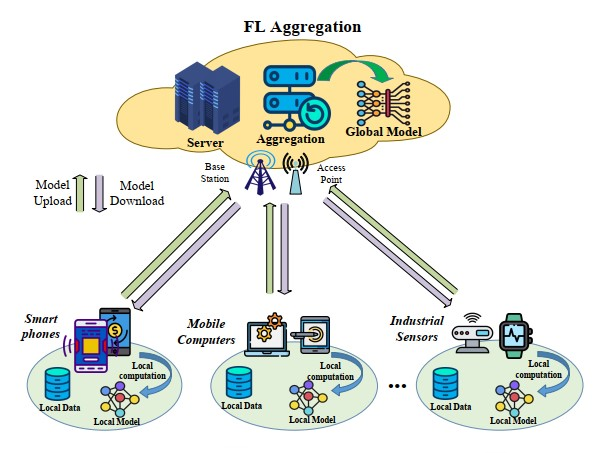
\includegraphics[height=8cm,width=10cm]{./arch/FL_architecture.jpg}
\caption[معماری یک شبکه یادگیری فدرال]{ معماری یک شبکه یادگیری فدرال\cite{a10}}
\label{wt}
\centering
\end{figure}

\section{پیشینه تحقیق}

پژوهشگران فعال در حوزه یادگیری فدرال در حال حاضر بیشتر بر دو چالش اصلی تمرکز دارند. اولاً، ناهمگونی داده در بین کارگران باعث کند شدن همگرایی مدل نسبت به یادگیری سنتی می‌شود. چالش دیگر هزینه ارتباطی در هر دو فرآیند بارگذاری و بارگیری مدل است که گلوگاه یادگیری توزیع شده است. به‌ خصوص در مورد سناریوهایی با تعداد دستگاه‌های زیاد در اینترنت اشیاء، این چالش جدی‌تر است. تعداد زیادی از کارها برای مقابله با این دو چالش پیشنهاد شده‌اند که می‌توان آن‌ها را در دسته‌بندی الگوریتم‌های بهینه‌سازی و استراتژی‌های کارآمد ارتباطات طبقه‌بندی نمود\cite{book_1}\cite{edge1}\cite{edge2}.

به عنوان مثال از الگوریتم‌های بهینه‌سازی می‌توان به انواع بهینه‌سازی‌های سراسری و محلی که سعی می‌کنند با استفاده از الگوریتم‌های مختلف، مانند گرادیان کاهشی، نمونه‌برداری تصادفی، گرادیان کاهشی تصادفی و غیره، به روزرسانی‌های مدل را در سرور مرکزی همگرا کنند. این روش‌ها برای کاهش هزینه ارتباطات و افزایش سرعت یادگیری مفید هستند. از طرف دیگر، می‌توان به استراتژی‌های کارآمدتر اشاره کرد که سعی می‌کنند با استفاده از روش‌های مختلف، مانند هماهنگ‌سازی دوره‌ای، هماهنگ‌سازی تصادفی، هماهنگ‌سازی بر اساس شرط و غیره، زمان و شرایط ارسال به روزرسانی‌های مدل را تعیین کنند. این روش‌ها برای حل مشکلات ناشی از نامتقارن بودن داده‌ها و نامتعادل بودن توزیع داده‌ها بین گره‌های محلی مناسب هستند. پژوهش‌های مختلف در این زمینه عموماً بر روی یک یا ترکیبی از چند از این روش‌ها تمرکز دارند.

\section{اهداف و دستاوردهای تحقیق}

باتوجه به اهمیت بارز روش‌های نوین یادگیری ماشین در دنیای امروزه و به خصوص کاربرد آن در اینترنت اشیاء، در این پروژه، سعی شده تا با استفاده از ظرفیت پردازش لبه یک چارچوب یادگیری فدرال مناسب که در آن چالش ارتباطات و ناهمگونی داده‌ها تا حد خوبی مدیریت شده ارائه دهد. شبیه‌سازی این نظریه در چارچوب نرم‌افزار‌های مطرح شبیه‌سازی از جمله \lr{GNS3}\LTRfootnote{Graphical Network Simulator-3} و \lr{Flower} و غیره انجام شده و نتایج نشان دهنده موثر بودن این راهکار است.

\section{ساختار گزارش}

در ادامه، فصل دوم مروری بر مفاهیم پایه مورد نیاز برای این پروژه را در بر میگیرد. فصل سوم به تعریف مسئله، معرفی و بررسی کامل مدل پیشنهادی برای حل مسئله، داده ها و چهارچوب کاری پروژه خواهد پرداخت. در نهایت، فصل چهارم ارزیابی و جمع بندی کلی پروژه را دربرمی‌گیرد.
